\documentclass[12pt,a4paper]{article}

\input{../../preamble_files/packages}
\input{../../preamble_files/scriptr}
\input{../../preamble_files/siunits}
\input{../../preamble_files/vectors}
\input{../../preamble_files/figures}
\input{../../preamble_files/references}
\input{../../preamble_files/empheq}

\pagestyle{fancy}
\lhead{Richard Whitehill}
\chead{PHYS 631 -- HW V}
\rhead{04/28/22}
\cfoot{\thepage \hspace{1pt} of \pageref{LastPage}}

\newcommand{\prob}[2]{\textbf{#1)} #2}

\setlength{\parskip}{\baselineskip}
\setlength{\parindent}{0pt}

\begin{document}

\prob{6.13}{
Suppose the field inside a large piece of magnetic material is $\va{B}_{0}$, so that $\va{H}_{0} = \frac{1}{\mu_0}\va{B}_{0} - \va{M}$, where $\va{M}$ is a ``frozen-in'' magnetization.
}

\begin{figure}[H]
   \begin{center}
       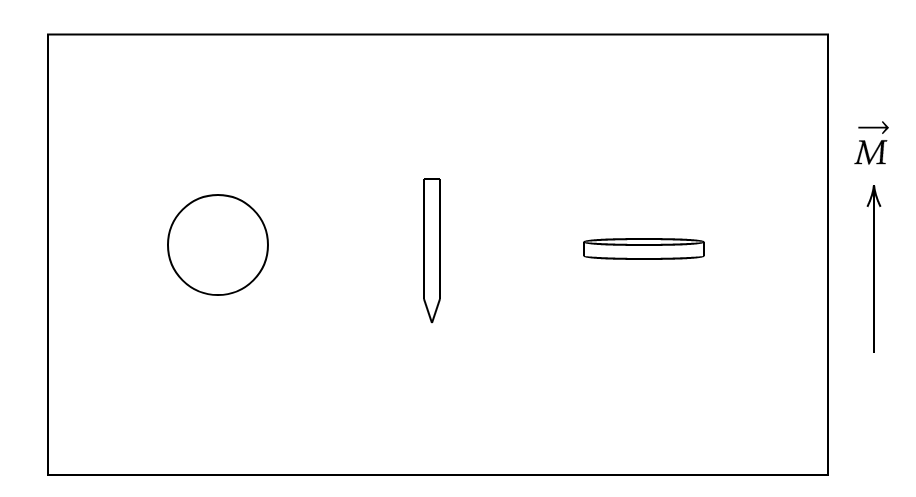
\includegraphics[scale=0.5]{./fig1.png}
   \end{center} 
\end{figure}

a) Now a small spherical cavity is hollowed out of the material.
Find the field at the center of the cavity, in terms of $\va{B}_{0}$ and $\va{M}$.
Also find $\va{H}$ at the center of the cavity, in terms of $\va{H}_{0}$ and $\va{M}$.

We know the magnetic field of a uniformly polarized sphere.
Here we can directly write the result since the cavity is ``made'' by inserting a material with magnetization $-\va{M}$:
\begin{eqbox}
    \va{B} = -\frac{2}{3} \mu_0 \va{M}
.\end{eqbox}
The auxiliary field is $\va{H} = \va{B}/\mu_0$ since the cavity has no net magnetization, meaning
\begin{eqbox}
    \va{H} = \frac{1}{\mu_{0}}\left( \va{B}_{0} - \frac{2}{3}\mu_{0}\va{M} \right) = \va{H}_{0} + \frac{1}{3}\va{M}
.\end{eqbox}

b) Do the same for a long needle-shaped cavity running parallel to $\va{M}$.

If we notice that there is no volume current density, then the only current density is that on the surface, and this setup can be approximated as a solenoid, giving us that
\begin{eqbox}
    \va{B} = -\mu_0 \va{M}
.\end{eqbox}
Thus, we have
\begin{eqbox}
    \va{H} = \frac{1}{\mu_0}\left( \va{B}_{0} - \mu_0 \va{M} \right) = \va{H}_{0}
.\end{eqbox}

c) Do the same for a thin wafer-shaped cavity perpendicular to $\va{M}$.

The thin wafer again has no volume bound current density, and the only bound surface current is the ring on the sides.
Thus, we can approximate the wafer as a ring of current, but we may suppose that the current is fairly weak, meaning that there is no magnetic field from magnetization.
\begin{eqbox}
    \va{B} = 0
.\end{eqbox}
Hence, we have
\begin{eqbox}
    \va{H} = \frac{1}{\mu_0}\va{B}_{0} = \va{H}_{0} + \va{M}
.\end{eqbox}

\prob{6.17}{
A current $I$ flows down a long straight wire of radius $a$.
If the wire is made of linear material (copper, say, or aluminum) with susceptibility $\chi_{m}$, and the current is distributed uniformly, what is the magnetic field a distance $s$ from the axis?
Find all the bound currents.
What is the \textit{net} bound current flowing down the wire?
}

\begin{figure}[H]
   \begin{center}
       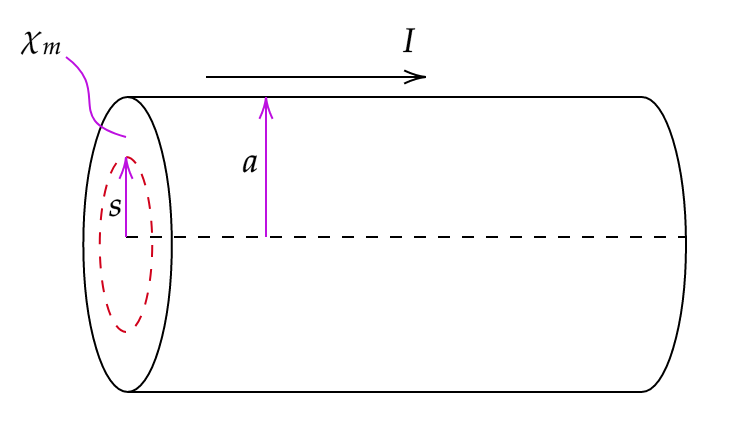
\includegraphics[scale=0.5]{./fig2.png} 
   \end{center} 
\end{figure}

In the wire, we have that the free current density
\begin{align*}
    \va{J}_{b} = \frac{I}{\pi a^2}
.\end{align*}
We can then find the auxiliary field using an amperian loop, which is circular of radius $s$:
\begin{align*}
    \oint \va{H} \vdot \dd{\va{l}} &= I_{\rm enc, f} \\
    H(2 \pi s) &= J \left( \pi s^2 \right) = \frac{s^2}{a^2}I \\
    H &= \frac{I}{2 \pi a^2} s
.\end{align*}
This allows us to write
\begin{eqbox}
    \va{B} = \mu \va{H} = \mu_0\left( 1 + \chi_{m} \right)\frac{I s}{2 \pi a^2}
.\end{eqbox}

Of course, this is only inside the wire.
Outside the total current enclosed is just $I$, so
\begin{eqbox}
    \va{B} = \mu_0 \va{H} = \frac{\mu_0 I}{2 \pi s}
.\end{eqbox}

The bound currents can be found as
\begin{align*}
    \va{J}_{b} &= \chi_{m} \va{J}_{f} = \frac{\chi_{m} I}{\pi a^2} \zhat \\
    \va{K}_{b} &= \va{M} \cross \shat = \chi_{m}\left( \va{H} \cross \shat \right) = -\frac{\chi_{m} I}{2 \pi a} \zhat 
.\end{align*}

If we add up the total volume and surface currents, then we have the net bound current as
\begin{eqbox}
    I_{b} = K_{b}\left( 2 \pi a \right) + J_{b}\left( \pi a^2 \right) = 0
.\end{eqbox}

\prob{6.21}{}

\begin{figure}[H]
   \begin{center}
       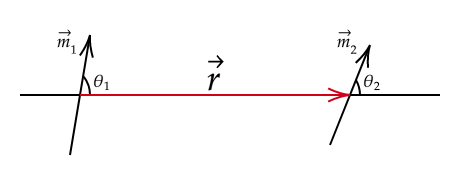
\includegraphics[scale=0.5]{./fig3.png} 
   \end{center} 
\end{figure}

a) Show that the energy of a magnetic dipole in a magnetic field $\va{B}$ is 
\begin{align*}
    U = -\va{m} \vdot \va{B}
.\end{align*}

The energy stored in the dipole is the same as the work needed to bring it into the position its in at any instant in time.
Any way that we construct the system should result in the same potential, so we will bring in the dipole perpendicular to the field and rotate it to an angle $\theta$ with the field.
Note that bringing the dipole in perpendicular to the field takes no work since $\va{F} = \grad{\va{m} \vdot \va{B}} = \grad{0} = 0$, so we are simply left with the work needed to bring the dipole to an angle $\theta$ with the field:
\begin{align*}
    W = \int_{\pi/2}^{\theta} \va{m} \cross \va{B} \dd{\theta} = mB \int_{\pi/2}^{\theta} \sin{\theta} \dd{\theta} = mB\left[ -\cos{\theta} \right]_{\pi/2}^{\theta} = -mB\cos{\theta} = -\va{m} \vdot \va{B}
.\end{align*}
Hence, the energy stored in the dipole is
\begin{eqbox}
    U = -\va{m} \vdot \va{B} 
\end{eqbox}

b) Show that the interaction energy of two magnetic dipoles separated by a displacement $\va{r}$ is given by
\begin{align*}
    U = \frac{\mu_0}{4 \pi}\frac{1}{r^3} \left[ \va{m}_{1} \vdot \va{m}_{2} - 3\left( \va{m}_{1} \vdot \rhat \right)\left( \va{m}_{2} \vdot \rhat \right) \right]
.\end{align*}

The interaction energy can either be found as the potential for $\va{m}_{1}$ in the field produced by $\va{B}_{2}$ or vice versa.
\begin{eqbox}
    U &= -\va{m}_{1} \vdot \va{B}_{2} = - \frac{\mu_0}{4 \pi}\frac{1}{r^3} \va{m}_{1} \left[ 3\left( \va{m}_{2} \vdot \rhat \right)\rhat - \va{m}_{2} \right] \\
      &= \frac{\mu_0}{4 \pi}\frac{1}{r^3}\left[ \va{m}_{1} \vdot \va{m}_{2} - 3\left( \va{m}_{1} \vdot \rhat \right)\left( \va{m}_{2} \vdot \rhat \right) \right]
.\end{eqbox}

c) Express your answer to (b) in terms of the angles $\theta_1$ and $\theta_2$, and use the result to find the stable configuration two dipoles would adopt if held a fixed distance apart, but left free to rotate.

We express the interaction energy in terms of angles using the basic geometric interpretation of the dot product:
\begin{eqbox}
    U &= \frac{\mu_0}{4 \pi}\frac{m_1 m_2}{r^3}\left[ \cos{\left( \theta_1 - \theta_2 \right)} - 3\cos{\theta_1}\cos{\theta_2} \right] \\
      &=  \frac{\mu_0}{4 \pi}\frac{m_1 m_2}{r^3}\left[ \sin{\theta_1}\sin{\theta_2} - 2\cos{\theta_1}\cos{\theta_2} \right]
.\end{eqbox}

To find stable configurations for this setup we must have simultaneously that 
\begin{align*}
    \dv{U}{\theta_1} = \dv{U}{\theta_2} = 0
.\end{align*}
The stability conditions are then
\begin{align*}
    \begin{cases}
        2\cos{\theta_2} \sin{\theta_1} + \sin{\theta_2} \cos{\theta_1} = 0 \\
        2\cos{\theta_1} \sin{\theta_2} + \sin{\theta_1} \cos{\theta_2} = 0
    \end{cases}
.\end{align*}

Subtracting the two equations gives us
\begin{align*}
    \cos{\theta_1} \sin{\theta_2} + \cos{\theta_2} \sin{\theta_1} = 0
.\end{align*}
Recall that we cannot simultaneously have $\sin{\theta} = 0$ and $\cos{\theta} = 0$, so both terms must go to zero at the same time, implying 
\begin{align*}
    \cos{\theta_1} \sin{\theta_2} &= 0 \\
    \cos{\theta_2} \sin{\theta_1} &= 0
.\end{align*}

We then have the following possible cases:
\begin{enumerate}
    \item $\cos{\theta_1} = 0$ implies $\cos{\theta_2} = 0$, so the dipoles may look like $\uparrow \downarrow$, $\downarrow \uparrow$, $\uparrow \uparrow$, or $\downarrow \downarrow$
    \item $\sin{\theta_2} = 0$ implies $\sin{\theta_1} = 0$, so either the dipoles look like $\rightarrow \rightarrow$, $\leftarrow \leftarrow$, $\leftarrow \rightarrow$, or $\rightarrow \leftarrow$.
\end{enumerate}

Some of these cases may be somewhat redundant since we can rotate the setup by some angle to achieve an equivalent orientation.

We can find the most stable configuration by assesing the value of the potential in these cases,
In each case, the coefficient is the same, so we simply evaluate the terms involving the angles.
For the first case, the second term vanishes, and either $\theta_1 - \theta_2 = 0,\,\pi$, giving the bracketed term as $\pm 1$.
For the second case, the sines vanish, and the cosines evaluate to one, giving the bracketed term as either $\pm 2$.

It is clear then that the absolute minimum is achieved when
\begin{align*}
    U = \frac{\mu_0}{4 \pi}\frac{m_1m_2}{r^3}\left( -2 \right)
,\end{align*}
which occurs when the dipoles are parallel along the axis defining their angles: $\rightarrow \rightarrow$.

d) Suppose you had a large collection of compass needles, mounted on pins at regular intervals along a straight line.
How would they point (assuming the earth's magnetic field can be neglected)?

A stable configuration between all of them is when they are all aligned, but the most stable is that with the lowest potential, which is when they are all pointing along the line they are mounted on.
This is the most probable state to find the needles in.

\end{document}
